\chapter{Billiard-AI}
In diesem Kapitel werden der Versuchsaufbau, die gewählte Architektur und die umgesetzten Lösungen beschrieben.

\section{Aufbau}
% TODO: beschreiben

\subsection{Kamera}\label{kap:camera}

Als Kamera wurde eine Intel RealSense Depth Camera D435 verwendet \cite{intel:realsense_d435}.
Die intrinsischen Kameraparameter des Farbsensors wurden mithilfe des RealSense SDK 2.43.0 \cite{github:realsense_sdk}
ausgelesen. Beim Farbsensor handelt es sich um einen \emph{OmniVision OV2740} \cite{intel:realsense_d435_datasheet}.
Die Auflösungs des Sensors beträgt 1920x1080 und die Pixelgrösse beträgt \SI{1.4}{\micro\metre} \cite{omnivision:ov2740}.

Nachfolgend ist die allgemeine intrinsische Kameramatrix in \emph{column-major order} aufgeführt.
Siehe \cite{matlab:what_is_camera_calibration} für die Erläuterung der Parameter in \emph{row-major order}.

\begin{align}
    \begin{pmatrix}
    f_x & s   & c_x\\
    0   & f_y & c_y\\
    0   & 0   & 1
    \end{pmatrix}
\end{align}

Die konkreten Werte für die Brennweite $(f_x, f_y)$ [Pixel], das optische Zentrum $(c_x, c_y)$ [Pixel]
und der Schiefekoeffizient $s$ sind nachfolgend eingefügt.

\begin{equation}
\begin{pmatrix}
1375.68884 & 0          & 974.842407\\
0          & 1375.85425 & 539.362732\\
0          & 0          & 1
\end{pmatrix}
\end{equation}

Die Parameter für die Modellierung der radialen und tangentialen Verzerrung $k_1$, $k_2$, $k_3$, $p_1$, $p_2$ sind gemäss
RealSense SDK alle 0 und das verwendete Modell wird \emph{Inverse Brown-Conrady} genannt.





\section{Aufbau und Messung}\label{kap:aufbauMessung}
Die Kamera wie auch der Projektor werden mittels eines Baugerüsts über dem Tisch platziert. Dieses ermöglicht die nötige
Flexibilität, um die optischen Objekte unabhängig voneinander optimal auszurichten.
TODO: Bild einfügen

Der Tisch ist an den Seiten leicht schräg, was ein genaues Messergebnis verunmöglicht. Weiterhin ist er an den Kanten
nicht fest und kann leicht deformiert werden. Um diese Ungenauigkeitsfaktoren möglichst gering zu halten, wurden die
gegenüberliegenden Tischkanten mit je zwei Holzstücken (Abbildung \ref{fig:messung:tisch}, 1), deren Breite individuell
über einen Messschieber millimetergenau bestimmt wurde, ausgestattet. Nun kann die Distanz zwischen den Holzstücken
gemessen und anschliessend die Breite der Hölzer dazuaddiert werden. Die Messung selbst (Abbildung \ref{fig:messung:tisch}, 2 und 3)
wird über ein Laser-Messgerät\footnote{Die genauen Spezifikationen sind im Anhang \ref{anhang:messung:messgeraete} ersichtlich.}
durchgeführt. Die Messungenauigkeit wird mit $\pm 1.5mm$ angegeben. Die Abbildung \ref{fig:messung:tisch} zeigt die Messung in X-Richtung,
diese Messung wird ebenfalls in gleicher Art und Weise in Y-Richtung durchgeführt.
\begin{figure}[h!]
    \begin{center}
        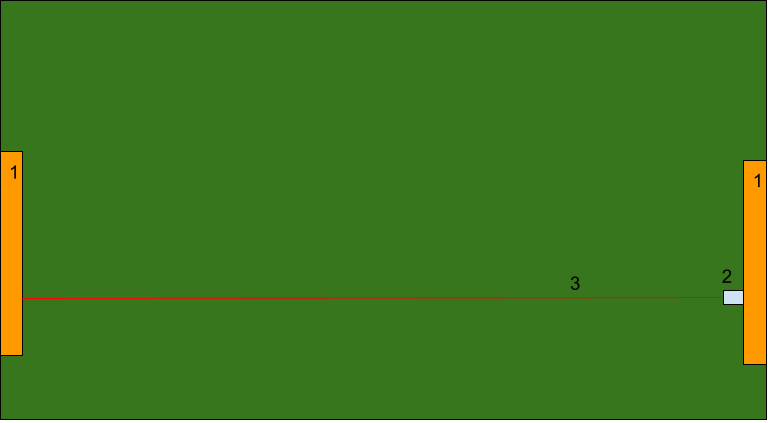
\includegraphics[width=0.8\linewidth]{../common/03_billiard_ai/resources/01_messung_tisch.png}
    \end{center}
    \caption{Messung - Tisch}
    \label{fig:messung:tisch}
\end{figure}


Um die Messung der Kugeln zu erläutern, muss zuerst das Koordinatensystem eingeführt werden. Die Kugeln selbst werden
über eine Kamera aufgenommen und deren Position daher auch in einem Pixelkoordinatensystem bestimmt. Dies ist aus
mehreren Gründen ungünstig. Einerseits soll die allgemeine Abhängigkeit zur Kamera vermieden werden, andererseits ist das
Pixelkoordinatensystem für die Visualisierung nicht gut geeignet.\\
Die Kugeln werden also in ein Modellkoordinatensystem übersetzt\footnote{Siehe Kapitel \ref{kap:model_coordinate_system}}.
Bei diesem befindet sich der Ursprung in der Mitte des Tisches und die X- wie auch die Y-Achse bilden die Breite und Höhe
in Millimeter ab.

Um nun die Position der Kugel zu bestimmen, wird zuerst deren Abstand zu den Banden gemessen (siehe Abbildung \label{fig:messung:kugel}, 1 und 2).
Dies geschieht wie beim Ausmessen des Tisches über ein Holzstück und das Lasermessgerät. Wurden beide Distanzen bestimmt, so
kann der Mittelpunkt der Kugel berechnet werden, indem noch der Radius, welcher durch einen Messschieber bestimmt wurde, dazuaddiert wird.
Es gilt nun, diesen Punkt in das Modellkoordinatensystem zu übersetzen. Dazu wird jeweils die halbe Breite wie auch Höhe
(beachte den Ursprung des Modellkoordinatensystems) von dem Mittelpunkt abgezogen. Abschliessend werden noch die korrekten
Vorzeichen über den Quadranten bestimmt.

\begin{figure}[h!]
    \begin{center}
        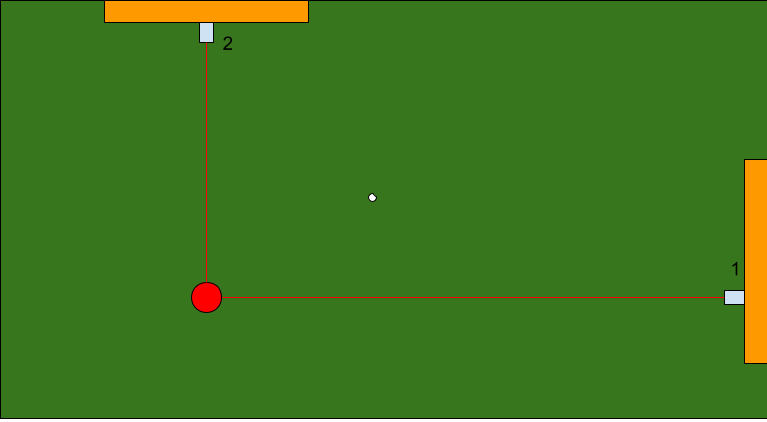
\includegraphics[width=0.8\linewidth]{../common/03_billiard_ai/resources/02_messung_kugel.png}
    \end{center}
    \caption{Messung - Kugel}
    \label{fig:messung:kugel}
\end{figure}

\section{Architektur}
Die eigentliche Funktionalität der Bildanalyse und Suche wird in einer Core-Library untergebracht, welche nativ in C++ entwickelt wird.
Die Anzeige der Hilfestellungen für den Spieler soll mithilfe von Unity erfolgen. Unity stellt die Schnittstelle zwischen
dem Spieler und der ganzen Applikation dar und muss sich daher mit der Core-Library austauschen.
Dafür wird eine C/C++-Bibliothek entwickelt, die ein C-Interface zur Core-Library bereitstellt.
Unity lädt diese Bibliothek und wandelt erhaltene native Objekte in Objekte um, welche in Unity verwendet werden können.
Eine Darstellung kann in Abbildung \ref{fig:top-level-architecture} entnommen werden.

\begin{figure}[h!]
    \begin{center}
        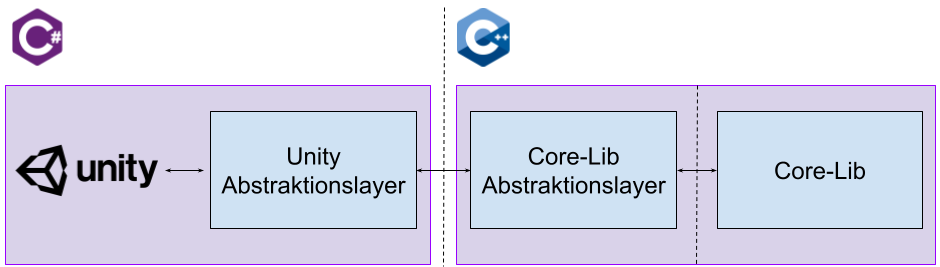
\includegraphics[width=0.8\linewidth]{../common/03_billiard_ai/resources/00_top_level_architecture.png}
    \end{center}
    \caption{Grobarchitektur - Applikationsumgebung}
    \label{fig:top-level-architecture}
\end{figure}

Die Core-Library selbst besteht aus den folgenden Komponenten:
\begin{description}
    \item[billiard\textunderscore capture] Dient als Schnittstelle zur Kamera und stellt die Bilder im OpenCV-Format bereit.
    \item[billiard\textunderscore detection] Erstellt aus dem Spielstand eine interne Repräsentation, welchen den Status beschreibt.
    \item[billiard\textunderscore snooker] Enthält Snooker-spezifische Funktionalität, u.a. die Erkennung der Snooker-Kugeln auf dem Billiardtisch.
    \item[billiard\textunderscore search] Verwendet den aktuellen Status wie auch eine zusätzliche Such-Beschreibung, um einen optimalen
    Stoss zu berechnen.
    \item[billiard\textunderscore physics] Stellt Funktionalität bereit, um physikalische Berechnungen durchzuführen.
\end{description}

Für die Umsetzung der Core-Library wird OpenCV\footnote{Siehe https://opencv.org} 5.4.2 verwendet.

\section{Modellkoordinatensystem}\label{kap:model_coordinate_system}

Bei der Aufnahme des Spielstandes über eine Kamera können die Kugeln im Bild erkannt und deren Zentrum, was der
Position entspricht, in Pixelkoordinaten im Bild ermittelt werden.
Die Pixelkoordinaten sind für die weitere Verarbeitung, sei es Analyse und Darstellung des Spielstandes oder Simulation
von Spielzügen, nicht geeignet. Es wird ein Koordinatensystem benötigt, welches möglichst unabhängig von der Auflösung,
Position und Blickrichtung der Kamera ist.

Idealerweise werden die Pixelkoordinaten in ein zu definierendes Koordinatensystem transformiert, welches für die weitere
Verarbeitung verwendet werden kann. Nachfolgend wird dieses Koordinatensystem das Modellkoordinatensystem genannt
und ist wie folgt definiert:
\begin{enumerate}
  \item Das Koordinatensystem ist zweidimensional.
  \item Der Ursprung befindet sich in der Mitte des Billiardtisches auf Höhe der Kugelmittelpunkte.
  \item Die X-Achse ist parallel zu der längeren Seite und die Y-Achse ist parallel zu der kürzeren Seite des Tisches.
  \item Die Länge eines Einheitsvektors entspricht 1\si{\milli\metre}.
\end{enumerate}

Diese Definition ist insofern praktisch, als dass die Banden und Löcher des Billiardtischs sehr einfach in diesem
Koordinatensystem definiert werden können.
In Abbildung \ref{fig:table_model_coordinate_system} ist der Ursprung und die Achsen des Koordinatensystems eingezeichnet.

\begin{figure}[h!]
    \begin{center}
    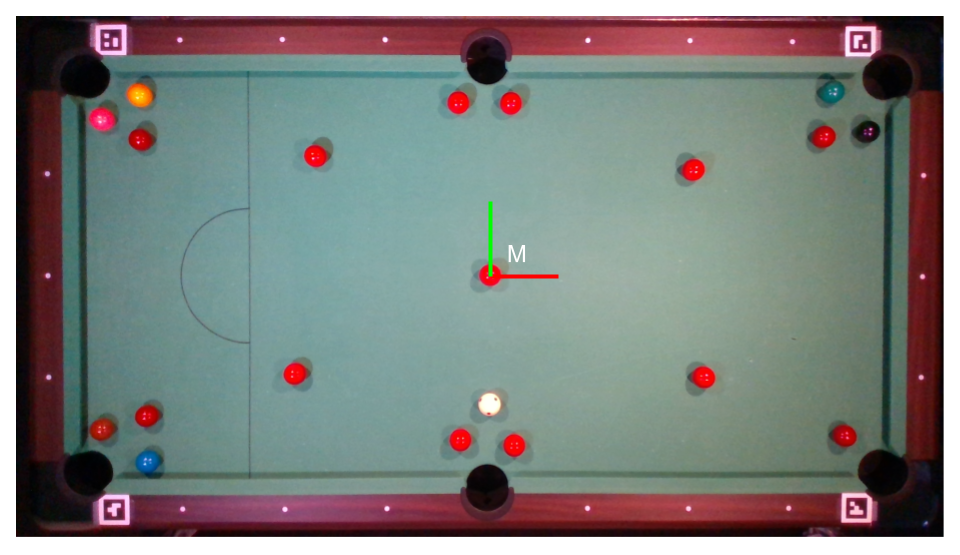
\includegraphics[width=0.8\linewidth]{../common/resources/coordinate_systems/table_model_coordinate_system.png}
    \end{center}
    \caption{Modellkoordinatensystem}
    \label{fig:table_model_coordinate_system}
\end{figure}

Die Transformation vom Pixelkoordinatensystem zum Modellkoordinatensystem erfolgt über mehrere Koordinatensystemtransformationen:
\begin{enumerate}
  \item \label{item:transforms_pixel_to_camera} Pixelkoordinaten zu Kamerakoordinaten, siehe Abschnitt \ref{kap:pixel_to_camera}
  \item \label{item:transforms_camera_to_world} Kamerakoordinaten zu Weltkoordinaten, siehe Abschnitt \ref{kap:camera_to_world}
  \item \label{item:transforms_world_to_rail} Weltkoordinaten zu Bandenkoordinaten, siehe Abschnitt \ref{kap:world_to_rail}
  \item \label{item:transforms_rail_to_model} Bandenkoordinaten zu Modellkoordinaten, siehe Abschnitt \ref{kap:rail_to_model}
\end{enumerate}

Alle Koordinatensysteme bis auf das Pixelkoordinatensystem sind in der Einheit Millimeter definiert,
um nicht benötigte Skalierungen in den Transformationen zu vermeiden.


\subsection{Pixelkoordinaten zu Kamerakoordinaten}\label{kap:pixel_to_camera}

Für die Transformation von Pixelkoordinaten zu Kamerakoordinaten wird die intrinsische Kameramatrix und
die Grösse der Sensorpixel der verwendeten Kamera benötigt.
Die intrinsische Kameramatrix $K$ ist nachfolgend erneut aufgeführt, diese wurde zusammen mit der
verwendeten Kamera in Abschnitt \ref{kap:camera} beschrieben.

\begin{align}
K =
\begin{pmatrix}
    f_x & s   & c_x\\
    0   & f_y & c_y\\
    0   & 0   & 1
\end{pmatrix}
\end{align}

Nun soll ein 2D-Punkt im Pixelkoordinatensystem in einen 3D-Punkt im Kamerakoordinatensystem überführt werden.
Sei der Pixelpunkt $p = (p_x, p_y)$, dann kann diesem der \emph{principal point} $c = (c_x, c_y)$ abgezogen werden, um den Ursprung in
die Mitte des Bildsensors zu verschieben. Anschliessend müssen die Koordinaten mit der
Sensorgrösse $s = (s_x, s_y)$ [\si{\milli\metre}] skaliert werden, um die Koordinaten von der Einheit Pixel
in die Einheit Millimeter umzuwandeln. Die Z-Komponente des resultierenden Punktes $P_C$ im Kamerakoordinatensystem ist
die Brennweite aus der intrinsischen Kameramatrix. Dabei gilt es zu beachten, dass die Parameter $f_x$ und $f_y$ der
intrinsischen Kameramatrix in der Einheit Pixel sind, und daher ebenfalls mit der Sensorgrösse $s$ skaliert werden müssen.

\begin{align}
f = f_x \cdot s_x\\
P_{C,x} = (p_x - c_x) \cdot s_x\\
P_{C,y} = (p_y - c_y) \cdot s_y\\
P_{C,z} = f\\
P_C = \begin{pmatrix}P_{C,x}\\P_{C,y}\\P_{C,z}\end{pmatrix}
\end{align}

Abbildung \ref{fig:camera_projection_learnopencv} zeigt das Bildkoordinatensystem und stammt
von \cite{learnopencv:geometry_of_image_formation},
wo eine ausführlichere Beschreibung der intrinsischen und extrinsischen Kameramatrix entnommen werden kann.

\begin{figure}[h!]
    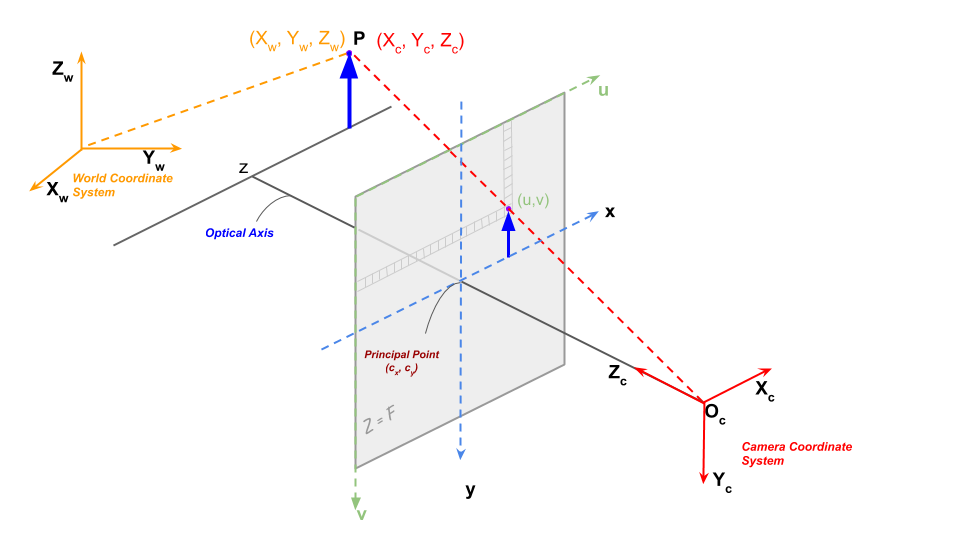
\includegraphics[width=0.8\linewidth]{../common/resources/coordinate_systems/camera_projection_learnopencv.png}
    \caption{Bildkoordinatensystem. Bildquelle: \cite{learnopencv:geometry_of_image_formation}}
    \label{fig:camera_projection_learnopencv}
\end{figure}

Damit ist diese Transformation abgeschlossen und der Punkt in Kamerakoordinaten kann in Weltkoordianten übersetzt werden.

\subsection{Kamerakoordinaten zu Weltkoordinaten}\label{kap:camera_to_world}

Der Punkt $P_C$ in Kamerakoordinaten muss nun in die reale Welt überführt werden. Da der Punkt $P_C$ relativ zur Kamera
positioniert ist, muss die Position der Kamera in der realen Welt bestimmt werden.
Somit braucht es eine \emph{pose estimation} der Kamera, d.h. die Position und Orientierung der Kamera in der realen Welt müssen bestimmt werden.
Eine \emph{pose estimation} benötigt eine kalibrierte Kamera und ein Objekt bekannte Grösse, welches im Bild erkannt werden kann.

Als Objekt bekannter Grösse und Position wurde ein ArUco-Board \cite{opencv:detection_of_aruco_boards} mit vier Markern verwendet.
Die verwendeten Marker mit einer Seitenlänge von 50\si{\milli\metre} und einer Grösse von 3x3 bits sind
in Abbildung \ref{fig:used_aruco_markers} aufgeführt.

\begin{figure}[h!]
    
\includegraphics[width=0.2\linewidth]{../common/resources/aruco/marker_0.png}
    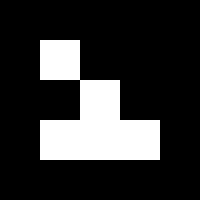
\includegraphics[width=0.2\linewidth]{../common/resources/aruco/marker_1.png}
    
\includegraphics[width=0.2\linewidth]{../common/resources/aruco/marker_2.png}
    
\includegraphics[width=0.2\linewidth]{../common/resources/aruco/marker_3.png}
    \caption{Verwendete ArUco markers}
    \label{fig:used_aruco_markers}
\end{figure}

Diese Marker wurden auf dem Tisch wie in Abbildung \ref{fig:table_with_aruco_markers} angebracht und deren relative
Position zueinander ausgemessen.

\begin{figure}[h!]
    \begin{center}
    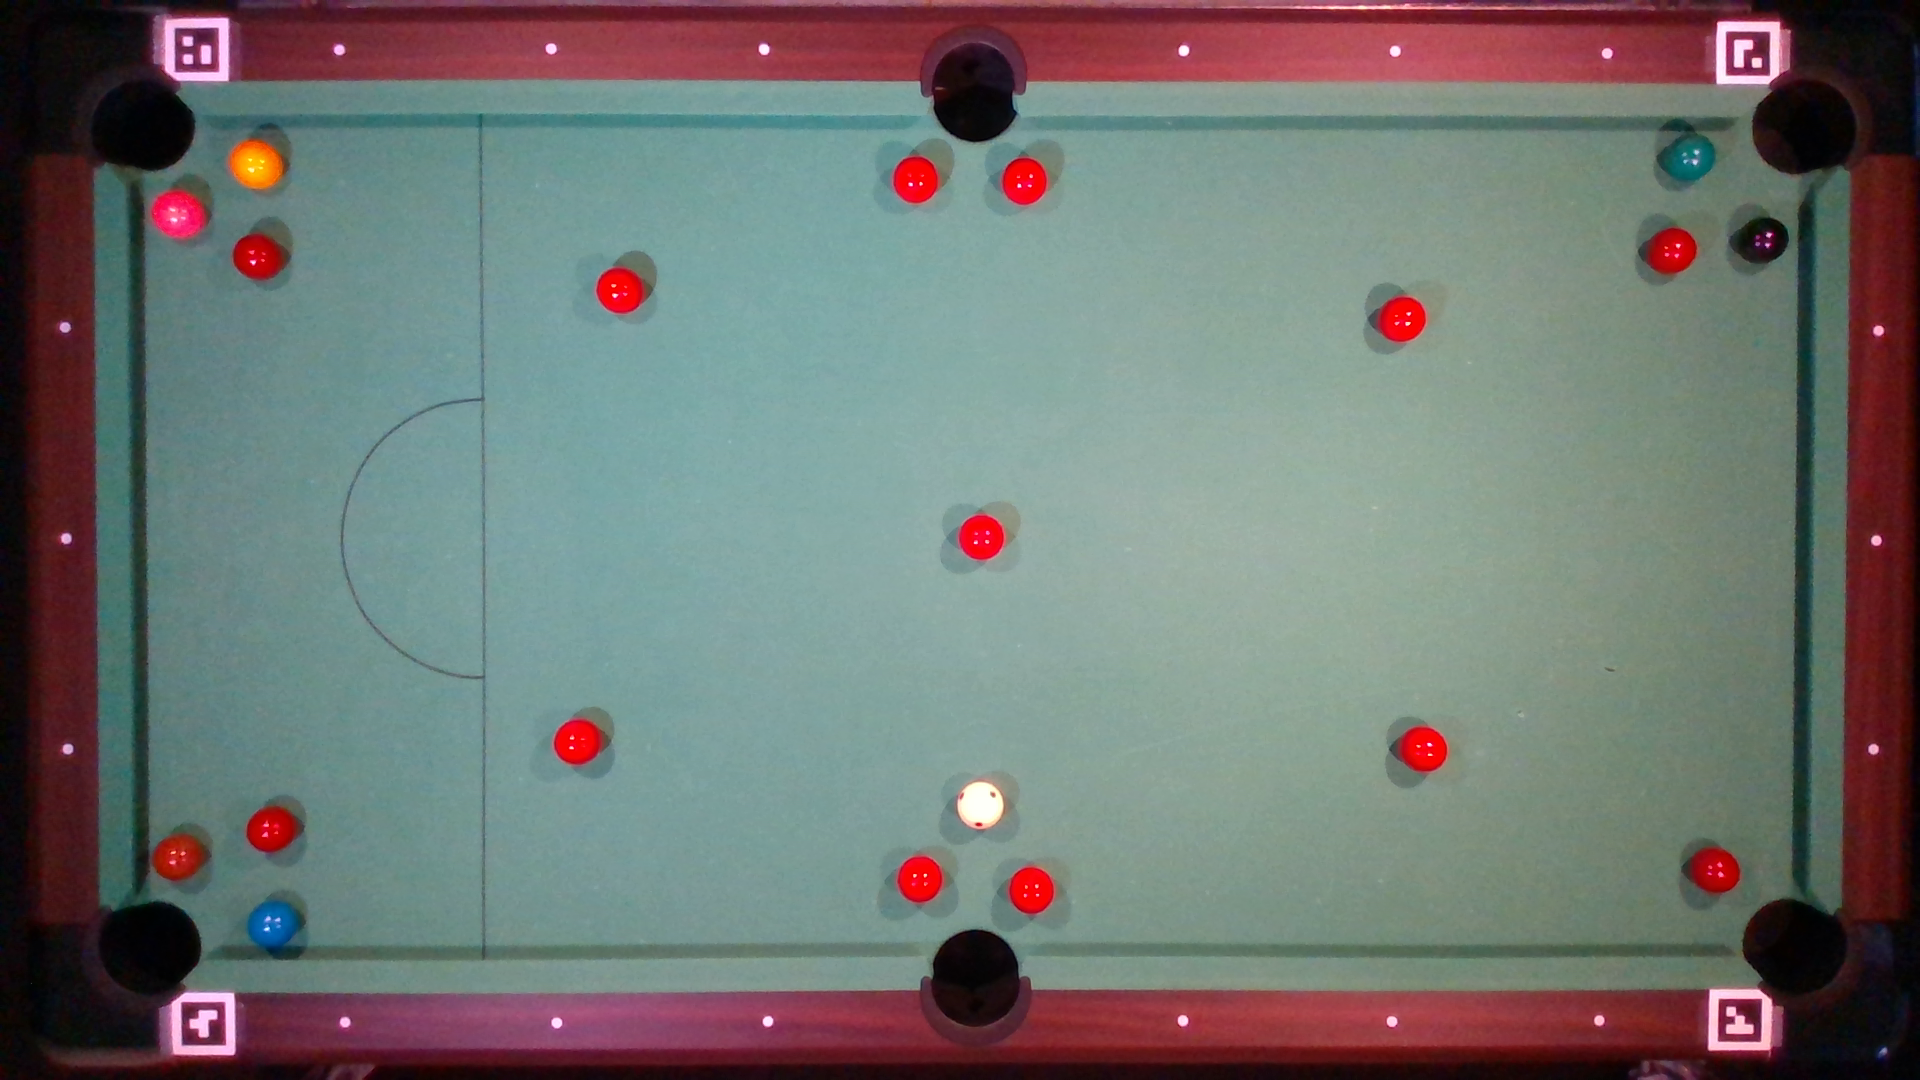
\includegraphics[width=0.6\linewidth]{../common/resources/coordinate_systems/table_with_markers.png}
    \end{center}
    \caption{Billiardtisch mit ArUco markers}
    \label{fig:table_with_aruco_markers}
\end{figure}

Das ArUco board ist definiert, sobald alle Eckpunkte der einzelnen Marker relativ zu einem
gewählten Weltkoordinatenursprung bekannt sind. Als Ursprung wurde der Mittelpunkt des Markers
in Abbildung \ref{fig:table_world_coordinate_system} unten links gewählt.
Die X-Achse ist parallel zur langen Seite des Tischs und die Y-Achse ist parallel zur kurzen Seite des Tischs.

\begin{figure}[h!]
    \begin{center}
    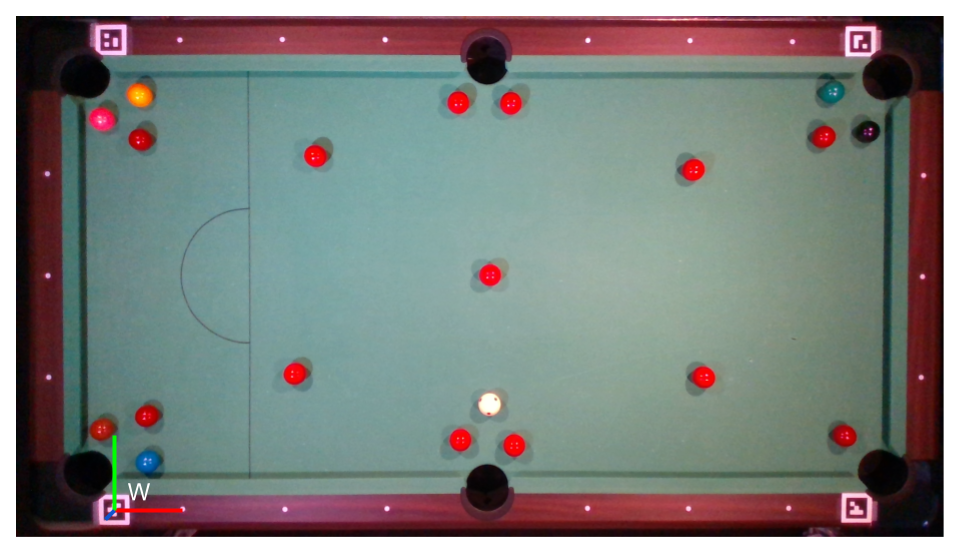
\includegraphics[width=0.6\linewidth]{../common/resources/coordinate_systems/table_world_coordinate_system.png}
    \end{center}
    \caption{Weltkoordinatensystem}
    \label{fig:table_world_coordinate_system}
\end{figure}

Mit der Definition des bekannten Objekts in der realen Welt kann nun die \emph{pose estimation} durchgeführt werden,
um daraus die extrinsische Kameramatrix zu bestimmen. Die extrinsische Kameramatrix $E$ beschreibt die Transformation eines
Punkts $P_W$ in Weltkoordinaten zu einem Punkt $P_C$ in Kamerakoordinaten und ist wie folgt definiert \cite{simek:extrinsic_camera_matrix}:

\begin{align}
E =
\begin{pmatrix}
    r_{1,1} & r_{1,2} & r_{1,3} & t_1\\
    r_{2,1} & r_{2,2} & r_{2,3} & t_2\\
    r_{3,1} & r_{3,2} & r_{3,3} & t_3\\
    0       & 0       & 0       & 1
\end{pmatrix}
\end{align}

Die inverse Transformation $E^{-1}$ transformiert einen Punkt $P_C$ in Kamerakoordinaten in einen Punkt $P_W$ in Weltkoordinaten.
So kann die Position der Kamera in Weltkoordinaten $C_W$ anhand der Position in Kamerakoordinaten $C_C$ und der Matrix $E^{-1}$ bestimmt werden:
\begin{align}
C_C = \begin{pmatrix} 0 \\ 0 \\ 0 \\ 1 \end{pmatrix}\\
C_W = E^{-1} \cdot C_C
\end{align}

Ebenso kann die Position des Pixels in Weltkoordianten $P_W$ bestimmt werden, wobei $P_C$
in Abschnitt \ref{kap:pixel_to_camera} erarbeitet wurde:

\begin{align}
P_C = \begin{pmatrix}P_{C,x}\\P_{C,y}\\P_{C,z}\end{pmatrix}\\
P_W = E^{-1} \cdot P_C
\end{align}

Es gilt zu beachten, dass die Position des Pixels in Weltkoordinaten $P_W$ nicht der Position des Kugel, welche evtl. an
dieser Pixelposition detektiert wurde, entspricht. Die projektive Abbildung der realen Welt auf den Bildsensor kann
nicht rückgängig gemacht werden, weil die Tiefeninformation verloren gegangen ist.

Da bekannt ist, dass sich alle Mittelpunkte der Kugeln auf dem Tisch auf einer Ebene befinden, kann die Pixelkoordinate
eines Kugelmittelpunkts trotzdem in eine Weltkoordinate transformiert werden.
Es gilt die Weltkoordinate $B_W$ der Kugel zu bestimmen.
Dazu kann eine Linie $L$ zwischen Kamera-Weltkoordinate $C_W$ und Pixel-Weltkoordinate $P_W$ gezogen werden und deren
Schnittpunkt mit der Ebene $\Sigma$, welche auf Höhe der Kugelmittelpunkte in Weltkoordinaten $H$ ist, bestimmt werden.
Die Linie $L$ ist in der Parameterform mit dem Stützvektor $\vec{q}$ und dem Richtungsvektor $\vec{v}$ und dem Skalierungsfaktor $\lambda$ definiert.
Sei $B$ eine Ebene in der Normalenform mit dem Stützvektor $\vec{a}$ und dem Normalenvektor $\vec{n}$, dann gilt:

\begin{align}
C_W = E^{-1} \cdot C_C\\
P_W = E^{-1} \cdot P_C\\
\vec{q} = C_W\\
\vec{v} = P_W - C_W\\
L: B_W = \vec{q} + \lambda \cdot \vec{v}\\
\vec{a} = \begin{pmatrix}0\\0\\H\end{pmatrix}\\
\vec{n} = \begin{pmatrix}0\\0\\1\end{pmatrix}\\
\Sigma: (B_W - \vec{a}) \cdot \vec{n} = 0\\
\end{align}

Durch Einsetzen der Liniengleichung in die Ebenengleichung kann der Schnittpunkt ermittelt werden.

\begin{align}
(\vec{q} + \lambda \cdot \vec{v} - \vec{a}) \cdot \vec{n} = 0\\
\vec{q} \cdot \vec{n} + \lambda \cdot \vec{v} \cdot \vec{n} - \vec{a} \cdot \vec{n} = 0\\
\lambda \cdot \vec{v} \cdot \vec{n} = \vec{a} \cdot \vec{n} - \vec{q} \cdot \vec{n}\\
\lambda \cdot \vec{v} \cdot \vec{n} = (\vec{a} - \vec{q}) \cdot \vec{n}\\
\lambda = \frac{(\vec{a} - \vec{q}) \cdot \vec{n}}{\vec{v} \cdot \vec{n}}
\end{align}

Falls $\vec{v} \cdot \vec{n} = 0$ gilt, dann gibt es keinen Schnittpunkt.
Die Kugel-Weltkoordinate kann durch Skalierung der Linie bestimmt werden:

\begin{align}
B_W = \vec{q} + \lambda \cdot \vec{v}\\
B_W = C_W + \lambda \cdot (P_W - C_W)\\
B_W = C_W + \frac{(\vec{a} - \vec{q}) \cdot \vec{n}}{\vec{v} \cdot \vec{n}} \cdot (P_W - C_W)
\end{align}

Damit ist die Weltkoordinate des Kugelmittelpunkts $B_W$ anhand dessen Pixel-Weltkoordinate $P_W$ ermittelt.


\subsection{Weltkoordinaten zu Bandenkoordinaten}\label{kap:world_to_rail}

Die vorletzte Transformation von Weltkoordinaten zu Bandenkoordinaten ist eine einfache Translation des Ursprungs,
siehe dazu Abbildung \ref{fig:table_world_to_rail}. Der Ursprung wird nicht rotiert, lediglich verschoben.
Diese Verschiebung kann auch in der Angabe der Weltkoordinaten des ArUco boards berücksichtigt werden, wodurch diese
Translation obsolet wird. Er wurde belassen, da dies eine kleine Operation darstellt und dadurch das Ausmessen des
ArUco boards und dessen Verschiebung zum Bandenursprung klar getrennt ist.

\begin{figure}[h!]
    \begin{center}
    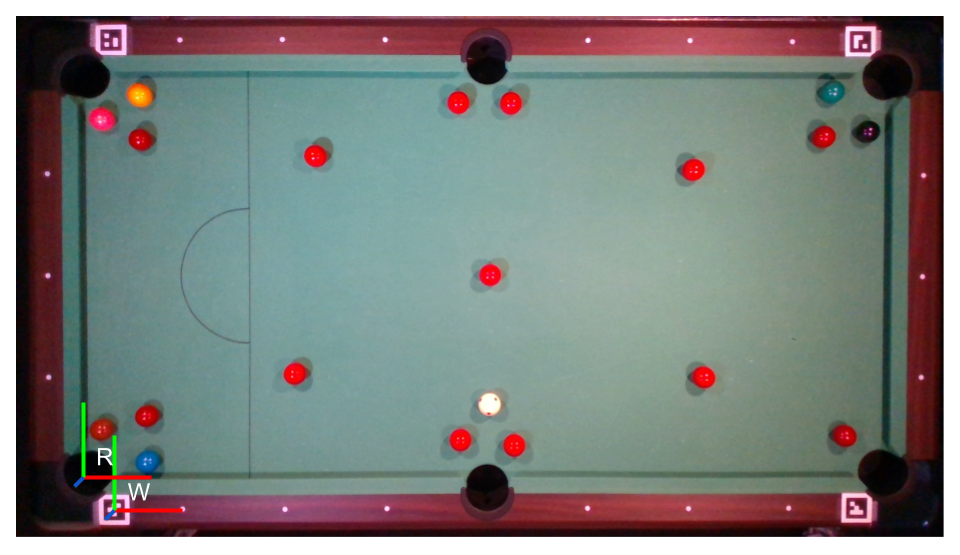
\includegraphics[width=0.6\linewidth]{../common/resources/coordinate_systems/table_world_to_rail.png}
    \end{center}
    \caption{Welt-Ursprung W und Banden-Ursprung R}
    \label{fig:table_world_to_rail}
\end{figure}

Wenn die Verschiebung von Welt-Ursprung zu Banden-Ursprung $T_{wb} = (\Delta x, \Delta y, 0)$ ist, dann ist
die Kugelposition in Bandenkoordinaten $B_R$:

\begin{align}
B_R = B_W + T_{wb}\\
B_R = B_W + \begin{pmatrix}\Delta x\\\Delta y\\0\end{pmatrix}
\end{align}

Somit steht nur noch die letzte Transformation bevor.


\subsection{Bandenkoordinaten zu Modellkoordinaten}\label{kap:rail_to_model}

Zuletzt wird der Ursprung erneut verschoben, vom Ursprung des Bandenkoordinatensystems zum
Ursprung des Modellkoordinatensystems, siehe dazu Abbildung \ref{fig:table_rail_to_model}.

\begin{figure}[h!]
    \begin{center}
    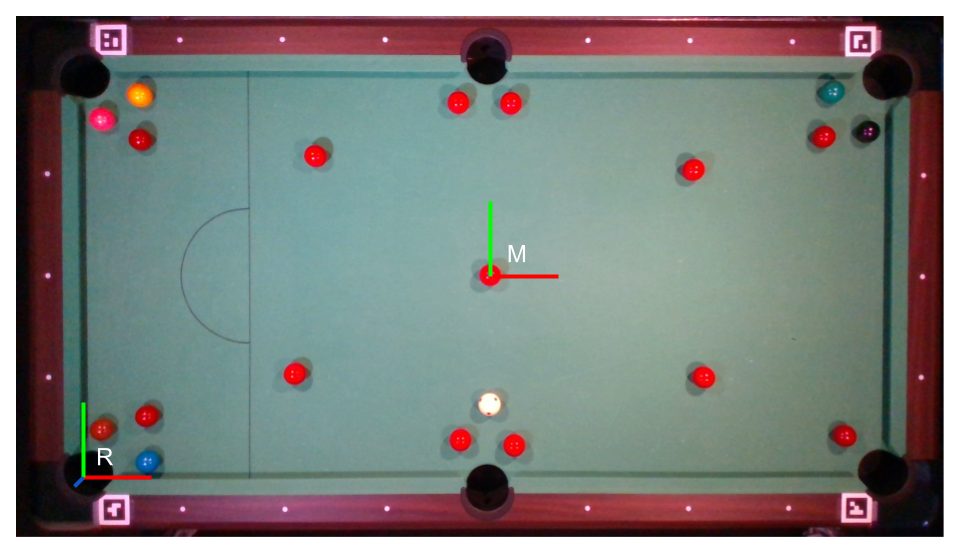
\includegraphics[width=0.6\linewidth]{../common/resources/coordinate_systems/table_rail_to_model.png}
    \end{center}
    \caption{Banden-Ursprung B und Modell-Ursprung R}
    \label{fig:table_rail_to_model}
\end{figure}

Für diese Verschiebung muss lediglich die Länge und Breite des Bereichs, welcher von den Banden begrenzt wird,
gemessen werden, siehe Abbildung \ref{fig:table_inner_lengths}.

\begin{figure}[h!]
    \begin{center}
    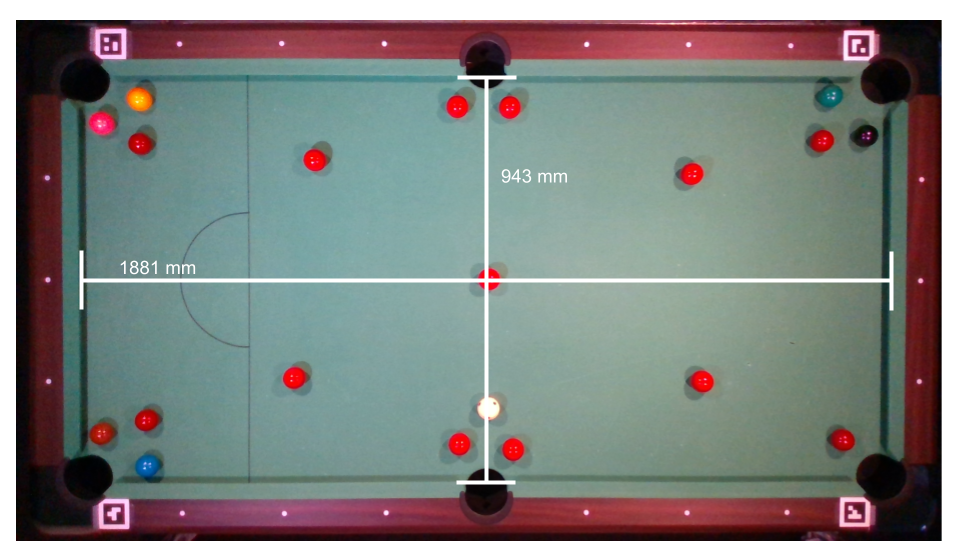
\includegraphics[width=0.6\linewidth]{../common/resources/coordinate_systems/table_inner_lengths.png}
    \end{center}
    \caption{Länge und Breite des Spielbereits}
    \label{fig:table_inner_lengths}
\end{figure}

Wenn der Spielbereich die Länge $L$ und Breite $B$ hat, dann ist die Kugelposition in Modellkoordinaten $B_M$:

\begin{align}
\Delta x = - \frac{L}{2}\\
\Delta y = - \frac{B}{2}\\
T_{bm} = \begin{pmatrix}\Delta x\\\Delta y\\0\end{pmatrix}
B_M = B_R + T_{bm}
\end{align}

Somit konnte die Kugelposition in Pixelkoordinaten in ein Modellkoordinatensystem umgewandelt werden, welches für
die weitere Verarbeitung von Nutzen ist.

\subsection{Modellkoordinaten zu Pixelkoordinaten}\label{kap:model_to_pixel}

Im Rahmen der Erkennung der Kugeln auf einem Bild ist es von Nutzen, die Pixlekoordinate einer Modellkoordinate
zu bestimmen. Beispielsweise kann der Radius der Kugeln in Pixel bestimmt werden, wenn die Länge des Tischs und der Radius
der Kugeln in Millimeter bekannt sind. Dies ist nützlich, da somit die genaue Pixelgrösse der Kugeln nicht fix hinterlegt sein muss.

Um dies zu bewerkstelligen, müssen einige der zu Beginn des Kapitels aufgeführten Transformationen rückgängig gemacht werden.
Die totwendigen Schritte sind die folgenden:
\begin{enumerate}
  \item Modellkoordinaten zu Bandenkoordinaten
  \item Bandenkoordinaten zu Weltkoordinaten
  \item Weltkoordinaten zu Kamerakoordinaten
  \item Weltkoordinaten zu Pixelkoordinaten
\end{enumerate}

Die Umwandlung von Modell- zu Bandenkoordinaten und von Banden- zu Weltkoordinaten sind die inversen Translationen, die
in den Abschnitten \ref{kap:rail_to_model}, resp. \ref{kap:world_to_rail}, beschrieben wurden.

Der Schritt von Welt- zu Pixelkoordinaten erfolgt direkt über die OpenCV-Funktion
\emph{projectPoints} \cite{opencv:projectPoints_function},
welche die extrinsische Kameramatrix, die intrinsische Kameramatrix und die Verzerrungskoeffizienten erfordert.
Im Prinzip wendet die Funktion die extrinsische, gefolgt von der intrinsischen Kameramatrix auf die Weltkoordinaten an,
führt die projektive Abbildung (\emph{perspective divide}) aus und wendet die Verzerrung an, um Pixelkoordinaten zu erhalten.

\subsection{Kugelradius in Pixel}\label{kap:ballradius_in_pixel}

Mithilfe des in Abschnitt \ref{kap:model_to_pixel} beschriebenen Algorithmus kann eine Modellkoordinate
in eine Pixelkoordinate überführt werden.
Der Radius der Kugel in Millimeter und die Länge des Spielbereichs (Länge zwischen den zwei kürzeren Banden) in Millimeter
können genutzt werden, um den Pixelradius der Kugel zu bestimmen.
Dazu werden zwei Punkte des Modellkoordinatensystems gewählt, $R_1$ und $R_2$, welche auf den gegenüberliegenden Banden
im Abstand $L$ liegen.
Sei $f(P_M)$ die Funktion, welche eine Modellkoordinate in eine Pixelkoordinate übersetzt,
dann gilt für den Kugelradius $x$ in Pixel:

\begin{align}
l = \frac{L}{2}\\
R_1 = \begin{pmatrix}-l\\0\\0\end{pmatrix}\\
R_2 = \begin{pmatrix}l\\0\\0\end{pmatrix}\\
P_1 = f(R_1)\\
P_2 = f(R_2)\\
\lambda = \frac{P_2 - P_1}{L}
x = R \cdot \lambda
\end{align}

Dabei handelt es sich bei $\lambda$ um den Faktor Pixel pro Millimeter.


\section{Detektion von Snooker-Kugeln}\label{kap:snooker_detection}

Ziel ist es, die Position, d.h. den Kugelmittelpunkt, jeder Kugel in Pixelkoordinaten so genau wie möglich zu bestimmen.
Diese Pixelkoordinaten können anschliessend wie in Kapitel \ref{kap:model_coordinate_system} beschrieben in ein
Modellkoordinatensystem umgewandelt werden, welches für die weitere Verarbeitung genutzt werden kann.

Die Anwendung des Circle Hough transform \cite{circle_hough} für die Extraktion der Kugeln ist naheliegend, führt allerdings auf dem
Graustufenbild dazu, dass auch Schatten als Kugeln detektiert werden. Diese gilt es zu vermeiden,
weshalb zunächst eine Segmentation aufgrund anderer Eigenschaften erfolgen muss.
In Abbildung \ref{fig:input_with_shadows} ist das Eingabebild mit Schatten abgebildet.

\begin{figure}[h!]
    \begin{center}
    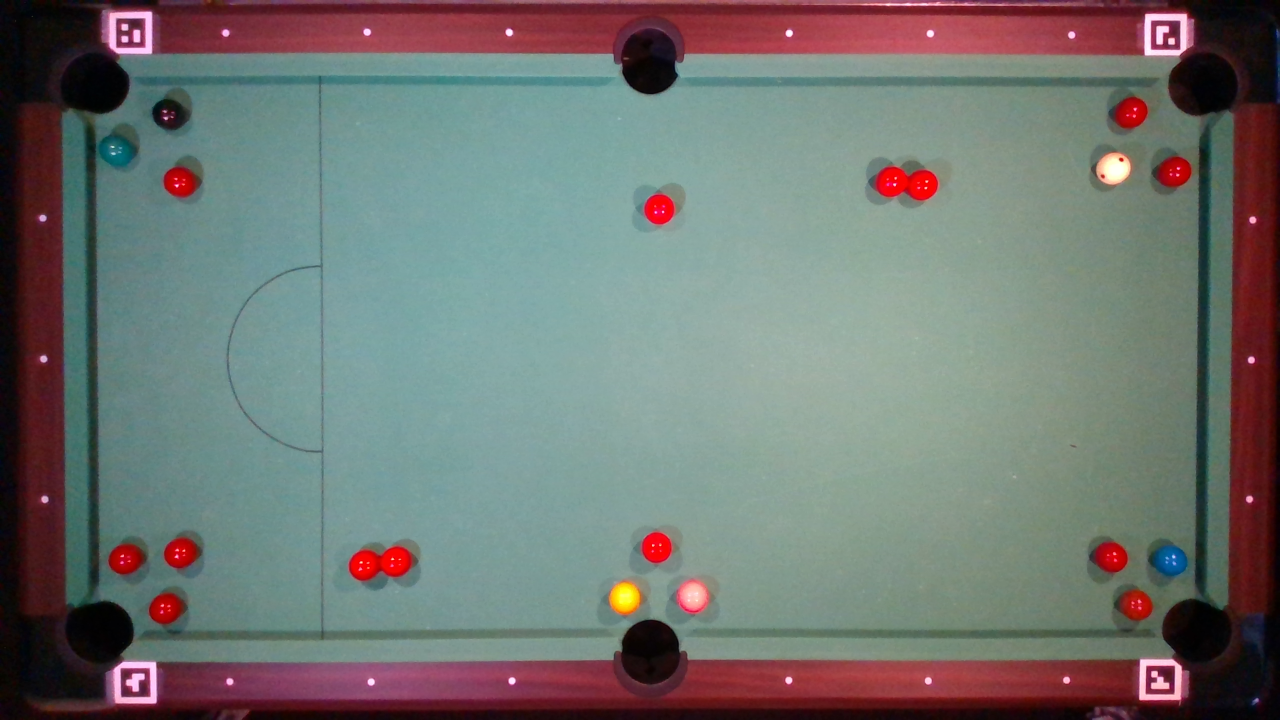
\includegraphics[width=0.8\linewidth]{../common/resources/detection/input.png}
    \end{center}
    \caption{Eingabebild mit Schatten}
    \label{fig:input_with_shadows}
\end{figure}

Zunächst wird ein Gaussfilter mit der Kernelgrösse von 5x5 auf das Eingabebild angewendet, um Rauschen zu unterdrücken.
Anschliessend wird das Bild vom RGB-Farbraum in den HSV-Farbraum \cite{hsv_color_space} umgewandelt, um eine einfacher
Segmentation zu ermöglichen, weil dadurch einzelne Eigenschaften wie Farbwert, Sättigung und Helligkeit gefiltert werden können.

Des weiteren sollen Kreise, welche ausserhalb des Spielfeld liegen, ausgeschlossen werden können.
Dazu wird eine binäre Maske, ein einkanaliges Bild mit den Werten 255 (= wahr) und 0 (= falsch), erzeugt.
In der Maske hat jedes Pixel, an dem ein Kugelmittelpunkt sein darf, den Wert 255, alle anderen den Wert 0.
Das Modellkoordinatensystem wurde in Kapitel \ref{kap:model_coordinate_system} beschrieben.
Die Banden und Löcher des Tisches können in Modellkoordinaten definiert werden, sofern der Tisch ausgemessen wurde.
In Kapitel \ref{kap:model_to_pixel} wurde erarbeitet, wie eine Modellkoordinate in eine Pixelkoordinate überführt werden kann.
Wird diese Transformation für alle Punkte der Banden und Löcher im Modellkoordinatensystem gemacht, können die
entstandenden Pixelpunkte in ein Bild eingezeichnet werden.
Somit kann eine binäre Maske erzeugt werden, welche lediglich das Spielfeld umfasst und damit den Rand des Tisches
und die Löcher aus einem Bild entfernen kann. In Abbildung \ref{fig:table_mask_applied} wurde diese Maske nach Anwendung
auf das Eingabebild aus Abbildung \ref{fig:input_with_shadows} dargestellt.

\begin{figure}[h!]
    \begin{center}
    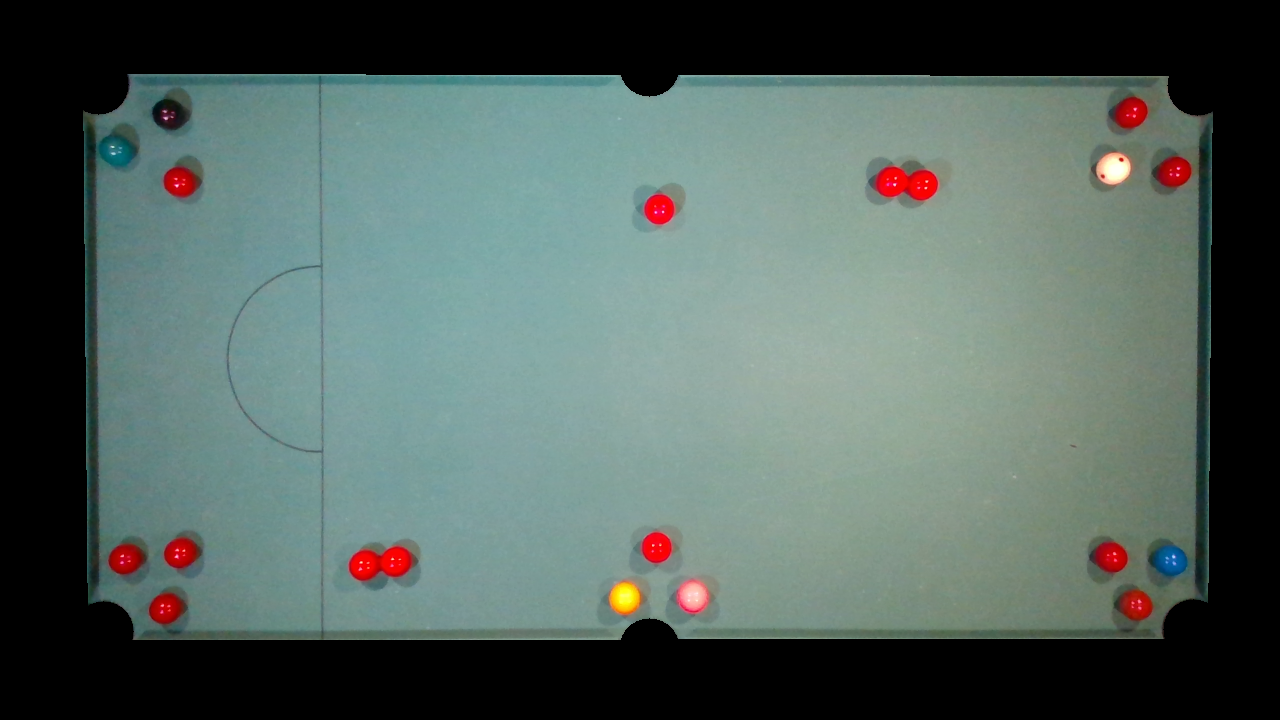
\includegraphics[width=0.8\linewidth]{../common/resources/detection/table_mask_applied.png}
    \end{center}
    \caption{Spielfeld-Maske. Zur Visualisierung auf Abbildung \ref{fig:input_with_shadows} angewendet.}
    \label{fig:table_mask_applied}
\end{figure}

In Snooker gibt es 22 Billiardkugeln, wovon 15 rot, und je eine weiss, schwarz, braun, gelb, grün, blau und pink sind.

Die Erkennung wurde wie folgt aufgeteilt:
\begin{itemize}
  \item Farbige Kugeln (rot, braun, gelb, grün, blau, pink)
  \item Weisse und pinke Kugel
  \item Schwarze Kugel
\end{itemize}

Die Segmentation der farbigen Kugeln erfolgt auf dem Sättigungskanal und diejenige der weissen und schwarzen Kugeln auf dem Helligkeitskanal des Bildes.
Eine Segmentation auf dem Farbwertskanal ist insbesondere für die grüne und blaue Kugel schwierig, weil der Billiardfilz grün ist
und dadurch die Grenze zwischen grünem Tisch und grüner Kugel zu wenig markant ist, siehe Abbildung \ref{fig:hue_green_table_problem}.

\begin{figure}[h!]
    \begin{center}
    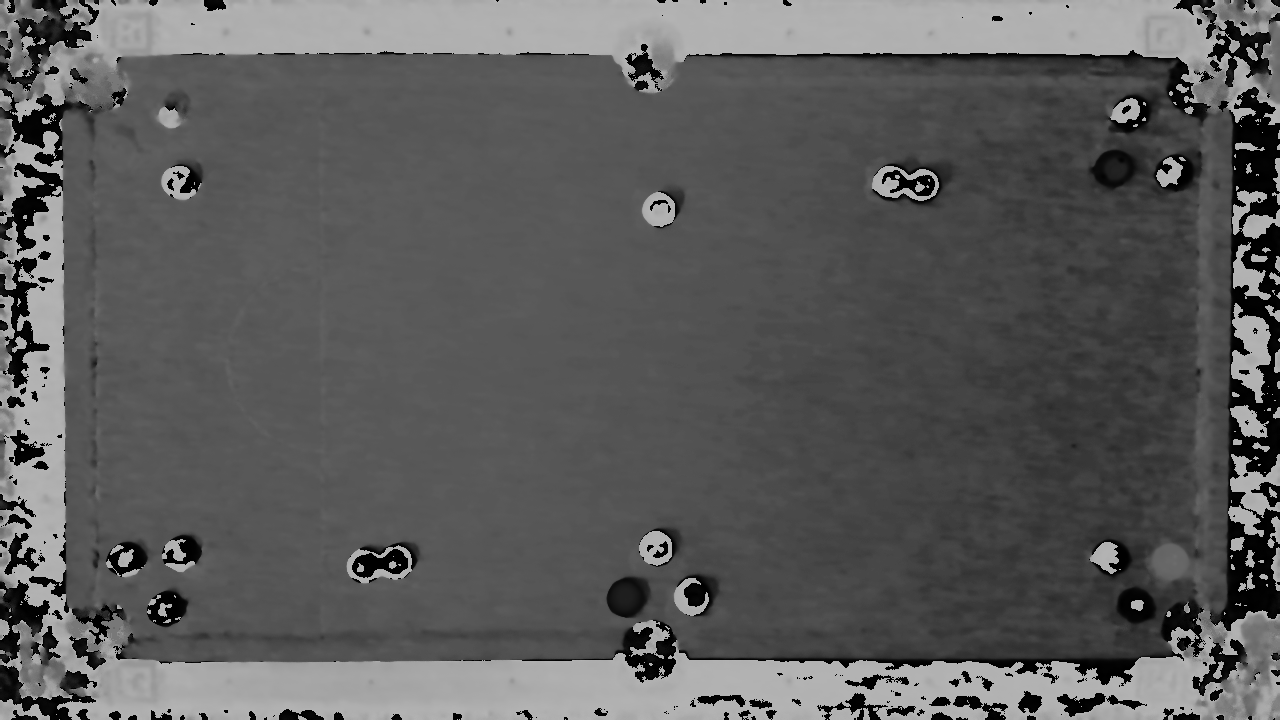
\includegraphics[width=0.8\linewidth]{../common/resources/detection/hue.png}
    \end{center}
    \caption{Der Farbwertskanal. Sehen Sie die grüne Kugel?}
    \label{fig:hue_green_table_problem}
\end{figure}

Die pinke Kugel ist insofern ein Spezialfall, als dass sie je nach Ausleuchtung eine stark gesättigte Farbe oder
eine grosse Helligkeit, ähnlich der weissen Kugel, aufweist. Das bedeutet, dass sie potentiell sowohl aufgrund
der Sättigung als auch der Helligkeit segmentiert wird und dadurch doppelt detektiert wird. Dies gilt es zu verhindern.

Für die Klassifikation der Kugeln, also die Bestimmung der Farbe der Kugel, ist der Farbwert trotzdem sehr sinnvoll.
Die Klassifikation wurde allerdings im Rahmen dieser Arbeit nicht vorgenommen.

Für alle nachfolgend beschriebenen morphologischen Operationen wird ein
rechteckiges structuring element der Grösse 3x3 Pixel verwendet.
Ausserdem ist der gesuchte Kugelradius in Pixel, welcher an den Hough transform übergeben wird, anhand des
Kugelradius in Millimeter berechnet, siehe dazu Kapitel \ref{kap:ballradius_in_pixel}.

Für die farbigen Kugeln mit hoher Sättigung wird ein Filter auf dem Sättigungskanal des HSV-Bilds
angewendet, um eine binäre Maske zu erhalten.

\begin{enumerate}
  \item Aufbau einer binären Maske mittels Filterung auf dem Sättigungskanal des HSV-Bilds.
  \item Morphologisches Opening der binären Maske, um kleine Störpixel zu entfernen.
  \item Morphologisches Closing der binären Maske, um kleine Löcher zu füllen.
  \item Anwendung der binären Maske auf das Graustufenbild, um alle unerwünschten Kugeln auszuschliessen.
  \item Canny edge detection \cite{canny_edge_detection} auf dem maskierten Graustufenbild, um ein Kantenbild zu erhalten.
  \item Hough transform auf dem Kantenbild, um Kreise zu erhalten.
  \item Verwerfen der Kreise mit Mittelpunkten ausserhalb der Spielfeld-Maske.
  \item Verwerfen der Kreise mit Mittelpunkten ausserhalb der binären Maske.
  \item Verwerfen der Kreise mit Mittelpunkten innerhalb der binären Maske der schwarzen Kugel.
\end{enumerate}

Die schwarze Kugel weisst eine geringe Sättigung und kann nicht aufgrund des Farbwerts segmentiert werden.
Das zuverlässigste ist demnach eine Filterung auf dem Helligkeitswert.
Die einzelnen Schritte der Detektion der schwarzen Kugel sind nachfolgend beschrieben:

\begin{enumerate}
  \item Aufbau einer binären Maske mittels Filterung auf dem Helligkeitskanal des HSV-Bilds.
  \item UND-Verknüpfung der binären Maske mit der binären Spielfeld-Maske, um die Löcher und den Rest des Tisches auszuschliessen.
  \item Morphologisches Closing der binären Maske, um kleine Löcher zu füllen.
  \item Morphologisches Opening der binären Maske, um kleine Störpixel zu entfernen.
  \item Anwendung der binären Maske auf das Graustufenbild, um alle unerwünschten Kugeln auszuschliessen.
  \item Canny edge detection auf dem maskierten Graustufenbild, um ein Kantenbild zu erhalten.
  \item Hough transform auf dem Kantenbild, um Kreise zu erhalten.
  \item Verwerfen der Kreise mit Mittelpunkten ausserhalb der Spielfeld-Maske.
  \item Verwerfen der Kreise mit Mittelpunkten ausserhalb der binären Maske.
\end{enumerate}

Die weisse Kugel weisst einen hohe Helligkeitswert auf, welcher zuverlässiger als der Sättigungswert gefiltert werden kann.
Nachfolgend ist der Ablauf der Detektion der weissen Kugel beschrieben.

\begin{enumerate}
  \item Aufbau einer binären Maske mittels Filterung auf dem Helligkeitskanal des HSV-Bilds.
  \item Morphologisches Opening der binären Maske, um kleine Störpixel zu entfernen.
  \item Morphologisches Closing der binären Maske, um kleine Löcher zu füllen.
  \item Anwendung der binären Maske auf das Graustufenbild, um alle unerwünschten Kugeln auszuschliessen.
  \item Morphologisches Closing des maskierten Graustufenbilds, da dadurch die roten Punkte,
  welche auf der weissen Kugel aufgemalt sind, schwächer werden.
  \item Canny edge detection auf dem maskierten Graustufenbild, um ein Kantenbild zu erhalten.
  \item Hough transform auf dem Kantenbild, um Kreise zu erhalten.
  \item Verwerfen der Kreise mit Mittelpunkten ausserhalb der Spielfeld-Maske.
  \item Verwerfen der Kreise mit Mittelpunkten ausserhalb der binären Maske.
  \item Verwerfen der Kreise mit Mittelpunkten innerhalb der binären Maske der farbigen Kugeln, um doppelt detektierte Kugeln, wie etwa die Pinke, zu vermeiden.
\end{enumerate}

Mithilfe der Maske für die weisse Kugel wird teilweise auch die pinke Kugel detektiert,
sofern diese eine geringe Sättigung und hohe Helligkeit aufweist.

Von den übriggebliebenen Kreisen werden die Mittelpunkte extrahiert und dienen als Resultat der Detektion.
Die detektierten Kreisradien sind irrelevant, da der Durchmesser der Kugeln bekannt ist.

Das Resultat der Zusammenführung der detektierten Kreise ist in Abbildung \ref{fig:hough_result} dargestellt.

\begin{figure}[h!]
    \begin{center}
    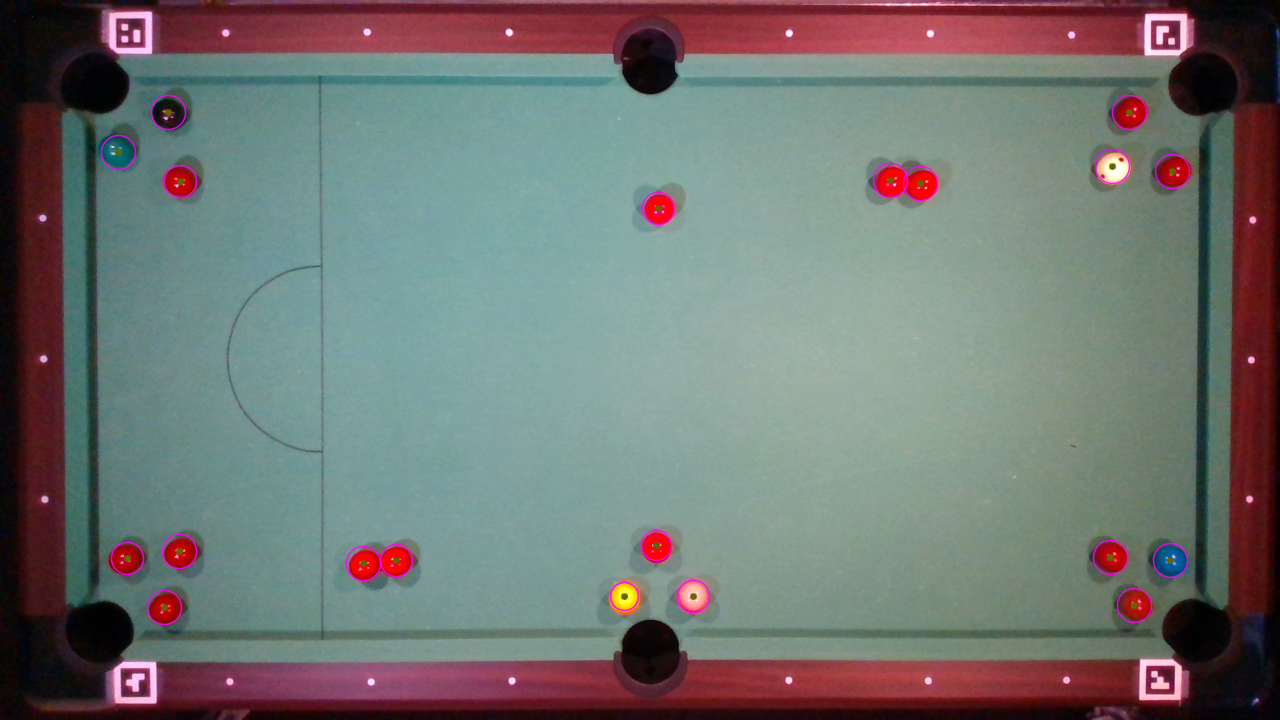
\includegraphics[width=0.8\linewidth]{../common/resources/detection/hough.png}
    \end{center}
    \caption{Resultat der Detektion. Die Kreismittelpunke und -umkreise sind eingezeichnet.}
    \label{fig:hough_result}
\end{figure}

